\chapter{Xenon Dynamics and Spatial Instability}
\label{ch:xenon}

Not all instabilities are fast. The slowest and most insidious arise from
$^{135}$Xe, a fission product with an enormous neutron-absorption cross-section
whose concentration lags the power by hours. Xenon dynamics produce the
post-shutdown ``dead time'' that constrains operation, and---in large cores---slow
spatial power oscillations. Both played a direct role at Chernobyl: it was xenon
poisoning, following an unplanned power drop, that lured the operators into
withdrawing nearly all the control rods, stripping the reactor of the shutdown
margin that might have saved it.

\section{The iodine--xenon chain}

$^{135}$Xe is produced in two ways: directly from fission (a small yield) and,
dominantly, from the beta-decay of its precursor $^{135}$I (half-life
$\sim 6.6\unit{h}$), which is itself a fission product (yield $\gamma_I\approx
6.4\%$). $^{135}$Xe is destroyed in two ways: by its own beta-decay (half-life
$\sim 9.2\unit{h}$) and by neutron capture---``burnup''---into $^{136}$Xe. Its
thermal absorption cross-section is about $2.6\times10^{6}\unit{barn}$, among the
largest known, so even trace amounts poison the reactor. The governing equations
are
\begin{align}
\frac{\dd I}{\dd t} &= \gamma_I \Sigma_f \phi - \lambda_I I,\\
\frac{\dd X}{\dd t} &= \gamma_X \Sigma_f \phi + \lambda_I I
                       - \lambda_X X - \sigma_X^a \phi\, X,
\end{align}
where $I$ and $X$ are the iodine and xenon concentrations, $\phi$ the flux, and
$\sigma_X^a$ the xenon absorption cross-section. The xenon contributes a negative
reactivity $\rho_X \propto -\sigma_X^a X$.

\section{Equilibrium xenon and its flux dependence}

At steady flux the concentrations reach equilibrium,
\begin{equation}
I_\infty = \frac{\gamma_I\Sigma_f\phi}{\lambda_I},\qquad
X_\infty = \frac{(\gamma_I+\gamma_X)\Sigma_f\phi}{\lambda_X + \sigma_X^a\phi}.
\end{equation}
At high flux, $\sigma_X^a\phi \gg \lambda_X$ and $X_\infty$ saturates: burnup
removes xenon as fast as it is made. The equilibrium xenon reactivity worth in a
high-power thermal reactor is large, of order a few per cent $\Delta k$---several
dollars---which must be compensated by control. The crucial nonlinearity is that
production of xenon (via iodine) depends on the \emph{past} flux, while burnup
depends on the \emph{present} flux; this time mismatch is the engine of every
xenon transient.

\section{The post-shutdown xenon peak and dead time}

Suppose the reactor is shut down (or its power sharply reduced) from a high flux.
Burnup of xenon ($\sigma_X^a\phi X$) stops immediately because $\phi$ collapses,
but the stockpiled iodine keeps decaying into xenon for hours. The xenon
concentration therefore \emph{rises} after shutdown, peaking several hours later
before the slower xenon decay finally wins and it falls. This transient buildup
adds a large negative reactivity---the ``xenon peak'' or ``iodine pit.'' If the
reactor's excess reactivity is insufficient to override the peak, it cannot be
restarted until the xenon decays: the \textbf{xenon dead time}, typically many
hours. Operators must either restart promptly (before the peak) or wait it out.

\begin{remark}[Chernobyl and the xenon trap]
On the night of 25--26 April 1986, the Chernobyl test was delayed and the reactor
power was held low and then dropped far below plan---down to about $30\unit{MW}$
thermal---for an extended period. Xenon built up and poisoned the core. To raise
power against the xenon, operators withdrew control rods far beyond the permitted
operating reactivity margin. The reactor was thus held critical only by a
dangerously small number of inserted rods, with most absorbers removed---a
configuration in which both the shutdown capability and the void coefficient were
at their worst. Xenon dynamics did not cause the explosion, but they set the
trap.
\end{remark}

\section{Spatial xenon oscillations}

In a physically large core---and the RBMK was very large, about $12\unit{m}$ in
diameter---the point approximation fails for slow phenomena, and xenon can drive
\emph{spatial} oscillations even at constant total power. The mechanism is a
delayed, out-of-phase feedback between flux and xenon:

\begin{enumerate}[nosep]
\item A perturbation raises the flux in one region (say, the top of the core) and
lowers it in another (the bottom).
\item In the high-flux region, xenon \emph{burns out} faster than it is produced,
so its concentration falls, which \emph{raises} the local reactivity and pushes
the flux even higher.
\item Meanwhile the extra iodine produced earlier in that region decays into
xenon hours later, eventually \emph{raising} the xenon and suppressing the flux
there---just as the other region, now iodine-rich, begins to flare.
\item The high-flux and low-flux regions thus trade places with a period of
roughly $15\!-\!30\unit{h}$.
\end{enumerate}

\begin{figure}[H]
\centering
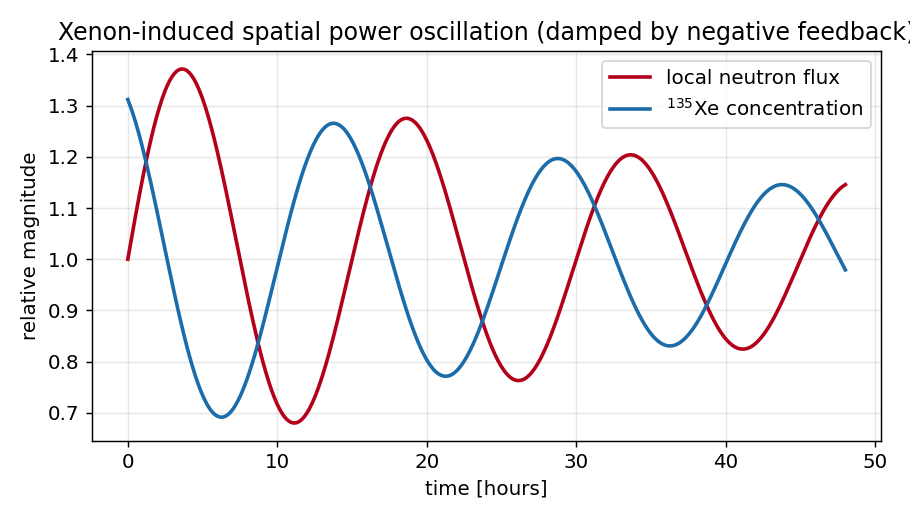
\includegraphics[width=0.82\linewidth]{figures/xenon.png}
\caption{Xenon-induced spatial power oscillation. The local flux and the
$^{135}$Xe concentration oscillate out of phase with a period of order a day. A
sufficiently negative power (temperature) coefficient damps the oscillation;
without it, the amplitude can grow.}
\label{fig:xenon}
\end{figure}

Whether these oscillations grow or decay depends on the power coefficient. A
strong \emph{negative} temperature/power coefficient damps them: as a region's
power rises, its temperature rises and removes reactivity, opposing the xenon-led
growth. A weak or positive coefficient leaves the oscillation undamped or growing.
Large reactors counter spatial xenon instability with negative feedback and with
spatial control (segmented control rods, flux mapping, and active power-shaping).
The RBMK required constant operator attention to its axial and radial power
distribution precisely because of its size and its marginal feedback; the night of
the accident, the flux shape was badly distorted (axially peaked), worsening the
local void and power coefficients beyond what core-average figures suggested.

\section{Implications for stability and operation}

Xenon dynamics teach two lessons relevant to thermal stability. First, the
reactor's state depends on its \emph{history}: the same power level can correspond
to very different xenon (and hence reactivity and rod) configurations depending on
what the power did over the preceding day. Operating procedures must account for
this memory. Second, spatial effects mean that a core can be ``stable on
average'' yet locally unstable; core-average coefficients can mislead. Both
lessons were violated at Chernobyl, where a history of power manoeuvring produced a
xenon-poisoned, rod-depleted, axially-distorted core whose local stability was far
worse than any single average number would suggest.

\keypoint{Xenon-135 introduces hours-long memory into reactor dynamics: a
post-shutdown poisoning peak that can preclude restart, and---in large cores---slow
spatial power oscillations damped only by negative feedback. At Chernobyl, xenon
poisoning drove the operators to strip out the control rods, creating the
low-margin, distorted-flux state in which the positive void coefficient could
trigger catastrophe.}



\section{Linear stability of the iodine--xenon equilibrium}
\label{sec:xenon-stability}

We now analyse xenon dynamics rigorously, first at a point (temporal stability)
and then for a spatial mode (the oscillation).

\paragraph{Temporal stability at fixed flux.}
Linearise the iodine--xenon equations about the equilibrium $(I_\infty,X_\infty)$
at constant flux $\phi_0$. With state $(\delta I,\delta X)$ the Jacobian is
\begin{equation}
\mathbf J=
\begin{pmatrix}
-\lambda_I & 0\\[2pt]
\lambda_I & -(\lambda_X+\sigma_X\phi_0)
\end{pmatrix},
\end{equation}
which is lower-triangular with eigenvalues $-\lambda_I<0$ and
$-(\lambda_X+\sigma_X\phi_0)<0$. Hence at fixed flux the point equilibrium is
\emph{unconditionally asymptotically stable}: a purely temporal xenon transient
(the post-shutdown peak) decays. Instability requires the flux to respond to
xenon, i.e.\ spatial coupling.

\paragraph{Spatial mode and the oscillation.}
Consider the first antisymmetric flux mode with amplitude $\epsilon(t)$ (a
``tilt'' between two halves of the core) coupled to the differential xenon
$\eta(t)$ and differential iodine $\zeta(t)$ between the halves. Retaining the
xenon reactivity feedback on the tilt and a prompt power (temperature) coefficient
$\alpha_P$, the linearised modal system takes the form
\begin{equation}
\dot\epsilon = g\,\big(c_X\,\eta + \alpha_P\,\epsilon\big),\quad
\dot\zeta = \gamma_I\Sigma_f\phi_0\,\epsilon-\lambda_I\zeta,\quad
\dot\eta = \lambda_I\zeta-(\lambda_X+\sigma_X\phi_0)\eta-\sigma_X\phi_0 X_\infty\,\epsilon,
\label{eq:xenon-modal}
\end{equation}
where $g>0$ is the modal flux gain and $c_X>0$ encodes the destabilising
xenon-burnout coupling. The Jacobian of \eqref{eq:xenon-modal} is $3\times3$ with
characteristic polynomial $s^3+b_1 s^2+b_2 s+b_3$ whose coefficients depend on
$\alpha_P$ through $b_1\ni -g\alpha_P$.

\begin{proposition}[Feedback threshold for spatial xenon stability]
\label{prop:xenon}
There is a critical coefficient $\alpha_{\rm crit}(\phi_0)>0$, increasing in the
flux $\phi_0$ and in the core size, such that the spatial xenon mode
\eqref{eq:xenon-modal} is asymptotically stable if and only if
\begin{equation}
\alpha_P < -\,\alpha_{\rm crit}(\phi_0).
\end{equation}
For $\alpha_P>-\alpha_{\rm crit}$ a complex-conjugate pair of eigenvalues crosses
into the right half-plane (a Hopf bifurcation), producing a growing oscillation
whose angular frequency at onset is
$\omega_{\rm osc}\approx\sqrt{b_2}$, corresponding to a period of order
$15$--$30\unit{h}$ for typical thermal-reactor parameters.
\end{proposition}
\begin{proof}[Sketch]
Apply the Routh--Hurwitz criterion (Theorem~\ref{thm:rh}) to
$s^3+b_1s^2+b_2s+b_3$. The destabilising xenon coupling enters $b_1,b_2,b_3$ with a
sign opposite to $\alpha_P$; a more negative $\alpha_P$ increases $b_1$ and the
product $b_1b_2-b_3$. The condition $b_1b_2-b_3>0$ defines a threshold
$\alpha_{\rm crit}$ such that the boundary $b_1b_2-b_3=0$ is the Hopf locus, where a
conjugate pair $s=\pm i\omega_{\rm osc}$ with $\omega_{\rm osc}^2=b_2$ sits on the
imaginary axis. The dependence of $\alpha_{\rm crit}$ on $\phi_0$ and core size
follows from $c_X,g\propto\phi_0$ and the larger spatial gain of bigger cores.
\end{proof}

Proposition~\ref{prop:xenon} formalises the qualitative claim of
Figure~\ref{fig:xenon}: a sufficiently strong negative power coefficient damps the
spatial xenon oscillation, while a weak or positive one permits a growing,
day-scale oscillation---most easily in a large core such as the RBMK.


\section*{Exercises}
\addcontentsline{toc}{section}{Exercises}
\begin{enumerate}[leftmargin=*,itemsep=2pt]
\item Write the iodine--xenon equations and find the equilibrium xenon concentration.
\item Explain why xenon \emph{builds up} after a shutdown from high power.
\item Describe the mechanism of spatial xenon oscillations and the role of negative feedback in damping them.
\item Explain how xenon poisoning contributed to the loss of operating reactivity margin at Chernobyl.
\item Why are large cores more susceptible to spatial xenon instability than small ones?
\end{enumerate}
